\chapter{Dátum- és időfüggvények}
\thispagestyle{empty}

A Függvénytündérben a dátum és idő kategóriát
választva olyan függvényeket találunk, melyek dátumok és
időpontok beszúrására, valamint szerkesztésére
szolgálnak. 

A \textbf{MA} függvény a rendszer dátumát adja
eredményül. A munkafüzetet megnyitva mindig aktualizálja az
értéket. Akkor is frissíti az értéket, amikor egy
cellaértéket módosítunk, vagy megnyomjuk az F9
funkcióbillentyűt. Szintaxisa: MA(), argumentuma nincs.

A \textbf{MOST} függvény a rendszer dátumát és idejét adja
eredményül. Minden esetben frissíti az értéket, amikor egy
cellaértéket módosítunk, vagy megnyomjuk az F9
funkcióbillentyűt.

A \textbf{DÁTUM} függvény kiszámítja az argumentumaiban év,
hónap, nap formában megadott dátumot. Alapértelmezett
formátuma a dátumformátum. Szintaxisa: DÁTUM(év;hónap;nap). A
hónapot és a  napot megadhatjuk lehetséges dátumon kívül
is. Ilyenkor átvitelre kerülnek a következő számjegyre. A
DÁTUM(2008;08;33) eredménye 2008-09-02 lesz.

A Calcban hat olyan függvény van, amelyek segítségével a
dátum- és időértékből azok részeit nyerhetjük ki. 
\Aref{DateFüggvények} táblázat ezeket mutatja be.

\begin{table}[!h]
\begin{center}
\caption{A dátum és az idő egyes részeinek kinyerése}\label{DateFüggvények}
\begin{tabular}{|m{2.5cm}|m{8cm}|}
\hline
ÉV &
Dátumértékből az évet adja vissza.\\ \hline
HÓNAP &
Dátumértékből a hónapot adja vissza.\\ \hline
NAP &
Dátumértékből a hónap napját (1-31) adja vissza.\\ \hline
ÓRA &
Időértékből az órákat adja vissza (0-23).\\ \hline
PERC &
Időértékből a perceket adja vissza (0-59).\\ \hline
MPERC &
Időértékből a másodperceket adja vissza (0-59).\\ \hline
\end{tabular}
\end{center}
\end{table}

A függvényeknek egy argumentumuk van, az átalakítandó dátum-
vagy időérték.

A \textbf{HÉT.NAPJA} függvény a dátumértéket a hét napjának
a sorszámaként adja vissza. Szintaxisa: HÉT.NAPJA(dátum;típus). A
\textbf{típus} argumentum a számítás módját határozza
meg. 1 esetén a hét napjai vasárnaptól számozódnak. 2
esetén a hét első napja a hétfő, 3 esetén pedig a
hétfő nullának (0) felel meg.

A \textbf{WEEKNUM} függvény egy dátumhoz tartozó hét
számát adja vissza. Szintaxisa:\\
WEEKNUM(dátum;mód). A mód
beállítja, hogy melyik legyen a hét első napja. Vasárnap
esetén értéke 1, hétfő esetén 2.

A \textbf{NETWORKDAYS} függvény két dátum közötti munkanapok
számát adja vissza. Szintaxisa: NETWORKDAYS(kezdő
dátum;befejező dátum;ünnepnapok). Az ünnepnapok a nem szombatra
vagy vasárnapra eső munkaszüneti napok listája. 

A \textbf{WORKDAY} függvény megadja azt a dátumot, amelyik egy
kezdő dátumhoz képest egy adott számú munkanapra
található. Szintaxisa: WORKDAY(kezdő
dátum;napok;ünnepnapok). Az ünnepnapok a nem szombatra
vagy vasárnapra eső munkaszüneti napok listája. 

Az \textbf{EASTERSUNDAY}\footnote{Az Excelben nem létezik.} függvénnyel az adott év Húsvét
vasárnapjának dátumát számíthatjuk ki. Szintaxisa:
EASTERSUNDAY(év).  Az \textbf{év} egy 1583 és 9956 közötti
évszám. E függvény segítségével más ünnepnapok is
kiszámíthatók egyszerű összeadás segítségével:

Húsvéthétfő = EASTERSUNDAY(év) + 1

Nagypéntek = EASTERSUNDAY(év) - 2

Pünkösdvasárnap = EASTERSUNDAY(év) + 49

Pünkösdhétfő = EASTERSUNDAY(év) + 50


\section{27. feladat}

{\itshape
Jelenítsük meg az ünnepek és emléknapok dátumait az A1
cellába beírt évben. Külön oszlopban jelenjen meg, hogy az
adott dátum milyen napra esik. A táblázat első sora az
évszám legyen, vagy szökőév esetén az ,,évszám -- szökőév''
felirat.}

Azt, hogy az adott év szökőév-e, meghatározhatjuk a DÁTUM
függvénnyel. Amennyiben a
{\sffamily\bfseries{HÓNAP(DÁTUM(A1;2;29))}} függvény értéke 2,
a DÁTUM függvény argumentuma
létező dátum. Tehát az A1 cellába írt évszám
szökőév. Ahhoz, hogy egy cellában az évszám vagy az
évszám és a szökőév szöveg jelenjen meg logikai
függvényt kell használnunk (\ref{27-feladatSzökőév} ábra).

\begin{figure}[!h]
\begin{center}
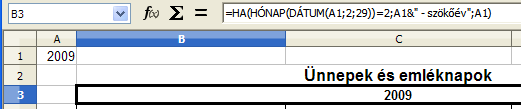
\includegraphics[width=13.783cm]{oocalcv2-img122.png}
\caption{27.  feladat --  szökőév}\label{27-feladatSzökőév}
\end{center}
\end{figure}

Azoknak az ünnepeknek a dátumát, amelyek egy bizonyos dátumra
esnek egyszerűen meghatározhatjuk a DÁTUM függvénnyel. Az
államalapítás ünnepét például a
{\sffamily\bfseries{=DÁTUM(A1;8;20)}} függvény adja meg.

\begin{figure}[!h]
\begin{center}
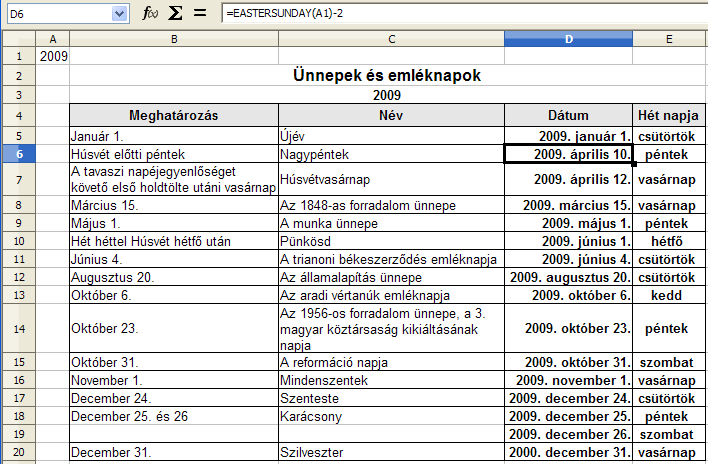
\includegraphics[width=15.999cm]{oocalcv2-img123.png}
\caption{27.  feladat -- DÁTUM függvény}\label{27-feladatDateFüggvény}
\end{center}
\end{figure}

A hét napját legegyszerűbben úgy határozhatjuk meg, hogy az
E5 cellába az =D5 képletet írjuk, a cella dátumformátumának
kódja pedig ,,nnnn'' lesz (\ref{27-feladatDateFüggvény} ábra). 


\section{28. feladat}

{\itshape
Magyarországon az Anyák napját május első vasárnapján
ünneplik. Határozzuk meg ezt a dátumot függvények
segítségével az A1 cellába írt évben.}

Az előző feladat táblázatában jelöljük ki az 10. sort
és szúrjunk be egy újat. A B10 és a C10 cellákba írjuk
\aref{28-feladatDATE} ábrán látható tartalmakat.

Május első vasárnapjának dátumának meghatározásához
tudnunk kell, hogy milyen napra esik május elseje. Ezt a
következő függvénnyel megtudhatjuk:
{\sffamily\textbf{HÉT.NAPJA(DÁTUM(A1;5;1);2)}}.
Értéke 1 lesz ha hétfőre, 2 ha keddre, 3 ha szerdára és
így tovább. Vasárnap esetén 7.

Az első vasárnap kiszámításához a május elsejei
dátumhoz 6-ot kell adni ha az hétfőre esik, 5-öt ha keddre,
4-et ha szerdára stb., ha vasárnapra esik akkor nullát. A
képlet tehát ez lesz (\ref{28-feladatDATE} ábra):
{\sffamily\textbf{=DÁTUM(A1;5;1)+(7-HÉT.NAPJA(DÁTUM(A1;5;1);2))}}.

\begin{figure}[!h]
\begin{center}
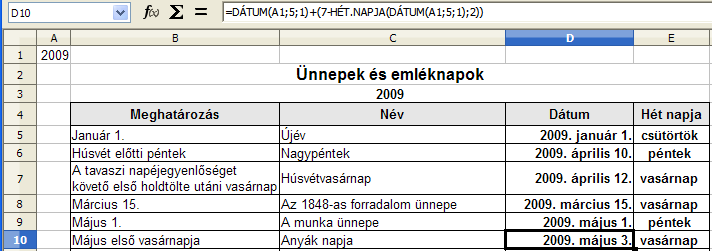
\includegraphics[width=15.999cm]{oocalcv2-img124.png}
\caption{28. feladat -- DÁTUM, HÉT.NAPJA függvények}\label{28-feladatDATE}
\end{center}
\end{figure}

Az ebben a fejezetben tárgyalt függvények \aref{14-fejezetFüggvények}
táblázatban láthatóak.

\begin{table}[!h]
\begin{center}
\caption{A fejezetben tárgyalt függvények}\label{14-fejezetFüggvények}
\begin{tabular}{|m{3cm}|m{8cm}|m{3cm}|}
\hline
\multicolumn{1}{|c|}{\textbf{A függvény}}&
\multicolumn{1}{c|}{\textbf{Funkciója}}&
\multicolumn{1}{c|}{\textbf{A függvény}} \\
\multicolumn{1}{|c|}{\textbf{neve}} & &
\multicolumn{1}{c|}{\textbf{angol neve}} \\
\hline
MA & A rendszer dátumát adja eredményül. & TODAY\\ \hline
MOST & A rendszer dátumát és idejét adja eredményül. & NOW\\ \hline
DÁTUM & Dátumértéket ad eredményül. & DATE\\ \hline
ÉV & Dátumértékből az évet adja vissza. & YEAR\\ \hline
HÓNAP & Dátumértékből a hónapot adja vissza. & MONTH\\ \hline
NAP & Dátumértékből a hónap napját adja vissza. & DAY\\ \hline
ÓRA & Időértékből az órákat adja vissza. & HOUR\\ \hline
PERC & Időértékből a perceket adja vissza. & MINUTE\\ \hline
MPERC & Időértékből a másodperceket adja vissza. & SECOND\\ \hline
HÉT.NAPJA & A hét napjának sorszámát adja vissza. & WEEKDAY\\ \hline
WEEKNUM & A dátumhoz tartozó hét számát adja meg. & WEEKNUM\\ \hline
NETWORKDAYS & Két dátum közötti munkanapok száma. & NETWORKDAYS\\ \hline
WORKDAY & Adott számú munkanappal későbbi dátum. & WORKDAY\\ \hline
EASTERSUNDAY & Egy adott évben a Húsvétvasárnap dátuma. & EASTERSUNDAY\\ \hline
\end{tabular}
\end{center}
\end{table}
